%%Introduction (chpt1)
\section{A brief history of drones}
\Glspl{uav} (Unmanned Aerial Vehicles), more commonly called drones, are defined as flying vehicles without human operators on board. They can be remote-controlled, or controlled by on-board computers. The earliest recorded use of \glspl{uav} dates back to 1849, when Austria launched about 200 unmanned balloons armed with bombs against de city of Venice \cite{anthology}. Due to unfavorable wind conditions, this attack failed, and the experiment was not repeated. The first functional UAVs were made towards de end of World War 1 and their use was, like the Austrian balloons, military. One example is the Kettering Bug (Figure \ref{fig:ketteringbug}), which was a torpedo with wings and a propeller developped by the US Army in 1918 \cite{dronesww1}.
\begin{figure}[H]
  \centering
  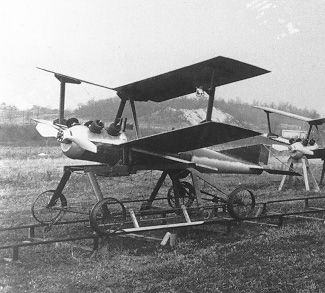
\includegraphics[width=0.5\textwidth]{kettering_bug.jpg}
    \caption{The Kettering Bug (1918)}
    \label{fig:ketteringbug}
\end{figure}

Throughout the 20th century, UAVs become more and more sophisticated, and were used more and more, but always for military purposes. In the more recent years, civilian UAVs have started to appear on the markets and their number quickly exceeded that of military UAVs. In february 2017, the FAA (Federal Aviation Administration) of the United States estimated that around 1.1 million units were in use in the US alone, and expected that number to rise to 3.55 million by 2021 \cite{consumerdronesbythenumbers}. These civilian drones are very different from military drones, in both their form and their function: civilian drones are usually smaller, and use rotors to take off vertically. They are used in a wide variety of applications.

\section{Motivation}
The ability to remote-control small and agile flying objects over large distances through the air, and to bring them to previously inaccessible locations, makes many new things possible. With the increasingly lower prices and better performances of civilian UAVs, people keep finding more and more uses for these high-tech gadgets. Some examples of these applications are: crop monitoring in agriculture \cite{agriculturaldrones}, delivery of mail or parcels, construction \cite{batiravecdesdrones}, cinematography, entertainment, or search and rescue operations. In all these applications, the more autonomous a drone is, the more efficient it will be at its task. One of the main challenges to achieve autonomy is for an UAV to be able to correctly identify its surroundings, and localize itself within them. In outdoor environments, GPS systems allow UAVs to know their position with great accuracy, but this is not possible in GPS-denied environments, such as indoors. The main subject of this thesis will be fully autonomous navigation by a quadcopter in a GPS-denied environment.

\subsection{Ethical considerations}
The new possibilities brought by drones also pose ethical questions about security and privacy. Even though this technology can improve people's quality of life, it also has the potential to diminish it. If drones start to be widely used comercially, we could reach a point where the sound nuisances that they cause seriously impacts people who live in densely populated areas. Also, they can make us feel less at home, knowing that we could be observed from the sky. For this reason, it is important to adopt strict reulations regarding the use of drones in public spaces. Fortunately, many countries are already adopting legislation in this direction.


\section{Context}
This thesis is part of a project at the UCL that spans over several years and several masters theses. This project was launched by professor Julien Hendrickx in the 2012-2013 academic year, and had as long-term goal to develop a program that would enable low-cost UAVs to navigate autonomously in indoor environments. This means creating a map of their environment, localizing themselves in this map, and avoidig obstacles during exploration, using only on-board sensors. Another goal is to allow several drones to collaborate to speed up exploration. Five theses have already been written on this subject, each taking the work of the previous a little further.
\paragraph{2012-2015: First three theses}
In each of the three academic years (2012-2013, 2013-2014, 2014-2015), one masters thesis on the subject of indoor navigation for autonomous low-cost drones was written. These masters theses formed the base of the future work. They implemented visual SLAM methods to allow drones to build a two-dimensional map based on keypoints (first red pucks, then visual landmarks that the drone detected from a textured field of view), and to localize itself within this map. During this time, inter-drone communication was also established, and was used to allow a drone to communicate the location of a target to another drone.

\paragraph{2015-2016: Recent work}
Last year, two groups of students simultaneously wrote theses on this subject. Before doing so, they joined forces to reimplement what had been done previously, but using the ROS interface, an interface to work with robots that would make many things simpler, and allow more flexibility (see section %%TODO for more).
The work of the first group of students allowed a drone to search and follow a mobile target, and call a second drone to continue this task when its battery was low.\\
The second group of students extended to SLAM algorithm to allow to use a 3D map to localize the drone. Unfortunately, they did not implement triangulation to allow to project seen points into 3D space, but rather made the assumption that all points were located on the ground when building the map. The end result was a drone capable of using a 3D map to localize itself, but not capable of building one from its observations.


\section{Objectives}
For my own thesis, my goal is to continue the work of last year's second group, to allow true 3-D SLAM: to build a 3D map based on observations by the monocular camera. To achieve this goal I will follow the following steps:
\begin{itemize}
\item Research the current state of the art for 3D Keyframe based monocular visual SLAM
\item Implement a way to triangulate points based on observations
\item Bundle Adjustment
\item Dense reconstruction
\item Obstacle Avoidance
\end{itemize}

\section{Ressources}

%%Hardware and software architecture (chpt3)
\subsection{Hardware}
For the practical implementation of this project, a Parrot AR.Drone 2.0 was used. This quadrotor was commercialized in 2012 and is an updated version of the original AR.Drone that was launched in 2010. This drone was marketed as a high tech toy, and is designed to be controlled from a smarphone application (connected to the drone via Wi-Fi). A few augmented reality games are available for the AR.Drone, in which it can visually recognise some predefined tags using its cameras, and interact with objects or other drones with a tag. To encourage the creation of more games for their drones, Parrot has released an open SDK that allows to effectively reprogram the drones. This early release of an open SDK has made it quite popular in the scientific community to do research on autonomous flight. The drone consists of 4 rotors, each with their own electric motor and microcontroller, an internal computer with a 1GHz ARM Cortex A8 processor and 1GB DDR2 RAM at 200MHz, and various sensors.

\subsubsection{Sensors}
The AR.drone has the following sensors:
\begin{itemize}
  \item 3 axis accelerometer with $\pm 50$ mg accuracy
  \item 3 axis gyroscope with $\pm 2000\degree/s$ accuracy
  \item Pressure sensor with $\pm 10 \texttt{Pa}$ accuracy
  \item 3 axis magnetometer with $\pm 6\degree$ accuracy
  \item Ultrasound sensor (facing downwards)
  \item Frontal camera (HD 720p 30fps)
  \item Ventral camera (QVGA, 60 fps)
\end{itemize}

The accelerometer and gyroscope together form the IMU.

\paragraph{Internal sensor fusion}
When remote-controlled during normal use, the internat controller needs a pose estimation to be able to stabilize itself. For safety reasons, it needs a reliable estimate of its altitude, and speeds, so that it can stop and hover. For convenience, it also needs a somewhat reliable estimation of its position, to cancel drifts when hovering. For these estimations, the internal controller fuses data from three sources: its IMU, its ultrasound sensor, and Odometry integrated from the optical flow observed by the bottom camera. Unfortunately, the values of these three sources ara available to be read from the drone, but not the internally fused pose, which is used directly by the controller.

\subsection{Software}

\subsubsection{Parrot SDK}
The SDK released by Parrot allows to send commands and receive information from the drone. However, it does not allow acces to code running in the drone during normal operation. It is possible to send the drone commands to take off, land, emergency stop, hover, move in a certain direction, but not to directly control the command send to the motors. Similarly, it is possible to read the IMU, ultrasound, odometry and video data from the drone, but not to access its own internal data fusion.

\subsubsection{ROS}
For the practical programming of the drone, the ROS (robot operating system) toolbox was used. This toolbox provides useful abstraction to program robots: the program is decomposed into "nodes", each node running simultaneously in a separate thread. Each node implements part of the drone's task, and the nodes can communicate between them by sending structured messages. The objective is to make the code modular, to be able to use existing nodes uploaded by other developpers. One such node, called "ardrone autonomy" created by %TODO
handles communication with a physical AR.Drone, so by using this node, we can completely disregard Parrot's specific SDK, and send all commands in ROS format. This way, we hope to make it easy to reuse code when changing hardware. ROS also provides a number of convenient tools for developping software to be used on robots: it provides ways to record and replay data, to easily set and change parameters, to run only specific parts of the program for testing.

\subsubsection{OpenCV}
OpenCV is an open-source computer vision library. It provides functions and data structures to manipulate images, and implements many state-of-the-art computer vision algorithms.

\subsubsection{PCL}
PCL stands for Point Cloud Library and is an open-source library for 3D point cloud processing. Currently is is only used to visualize the map created by the drone, but in the future, it can be used for higher-level functions on this map like combining maps created by multiple robots, or reconstructing a dense representation of the map from a point cloud.

\subsubsection{Ceres Solver}
Ceres solver is an open-source library for modeling and solving non-linear least squares problems. It will be used in this thesis to solve Bundle Adjustment problems.



\section{Outline}
First, the state of the art of %TODO
will be explored in chapter 2. Chapters 3 through 5 will present the main subject of this work: computer vision (Chapter 2), localisation (Chapter 3), Mapping (Chapter 5). The results will then be presented in chapters 6: Simultaneous Localisation and Mapping. Finally, we will conclude in chapter 7.
